\documentclass{lug}

\title{Computer Graphics \& OpenGL}
\author{Sam Sartor}
\institute{Mines Linux Users Group}

\usepackage{etoolbox}
\usepackage{array}
\usepackage{amsmath}
\usepackage{adjustbox}
\usepackage{calc}
\usepackage{lmodern}

\makeatletter
\patchcmd{\beamer@sectionintoc}{\vskip1.5em}{\vskip0.5em}{}{}
\makeatother

\newcommand{\pmidg}[1]{\parbox{\widthof{#1}}{#1}}
\newcommand{\splitslide}[4]{
    \noindent
    \begin{minipage}{#1 \textwidth - #2 }
        #3
    \end{minipage}%
    \hspace{ \dimexpr #2 * 2 \relax }%
    \begin{minipage}{\textwidth - #1 \textwidth - #2 }
        #4
    \end{minipage}
}

\begin{document}

\section{Introduction}

\begin{frame}{Uses}
    \splitslide{0.65}{.7em}{
        Computer graphics is everywhere!
        \begin{itemize}
            \item Your terminal
            \item Web browsers
            \item Video games
            \item CAD software
            \item Movies, TV Shows
            \item Virtual reality
            \item Your bootloader
            \item QT, GTK+, wxWidgets
            \item Vim, Emacs, Notepad
            \item Embedded devices
        \end{itemize}
    }{
        \pmidg{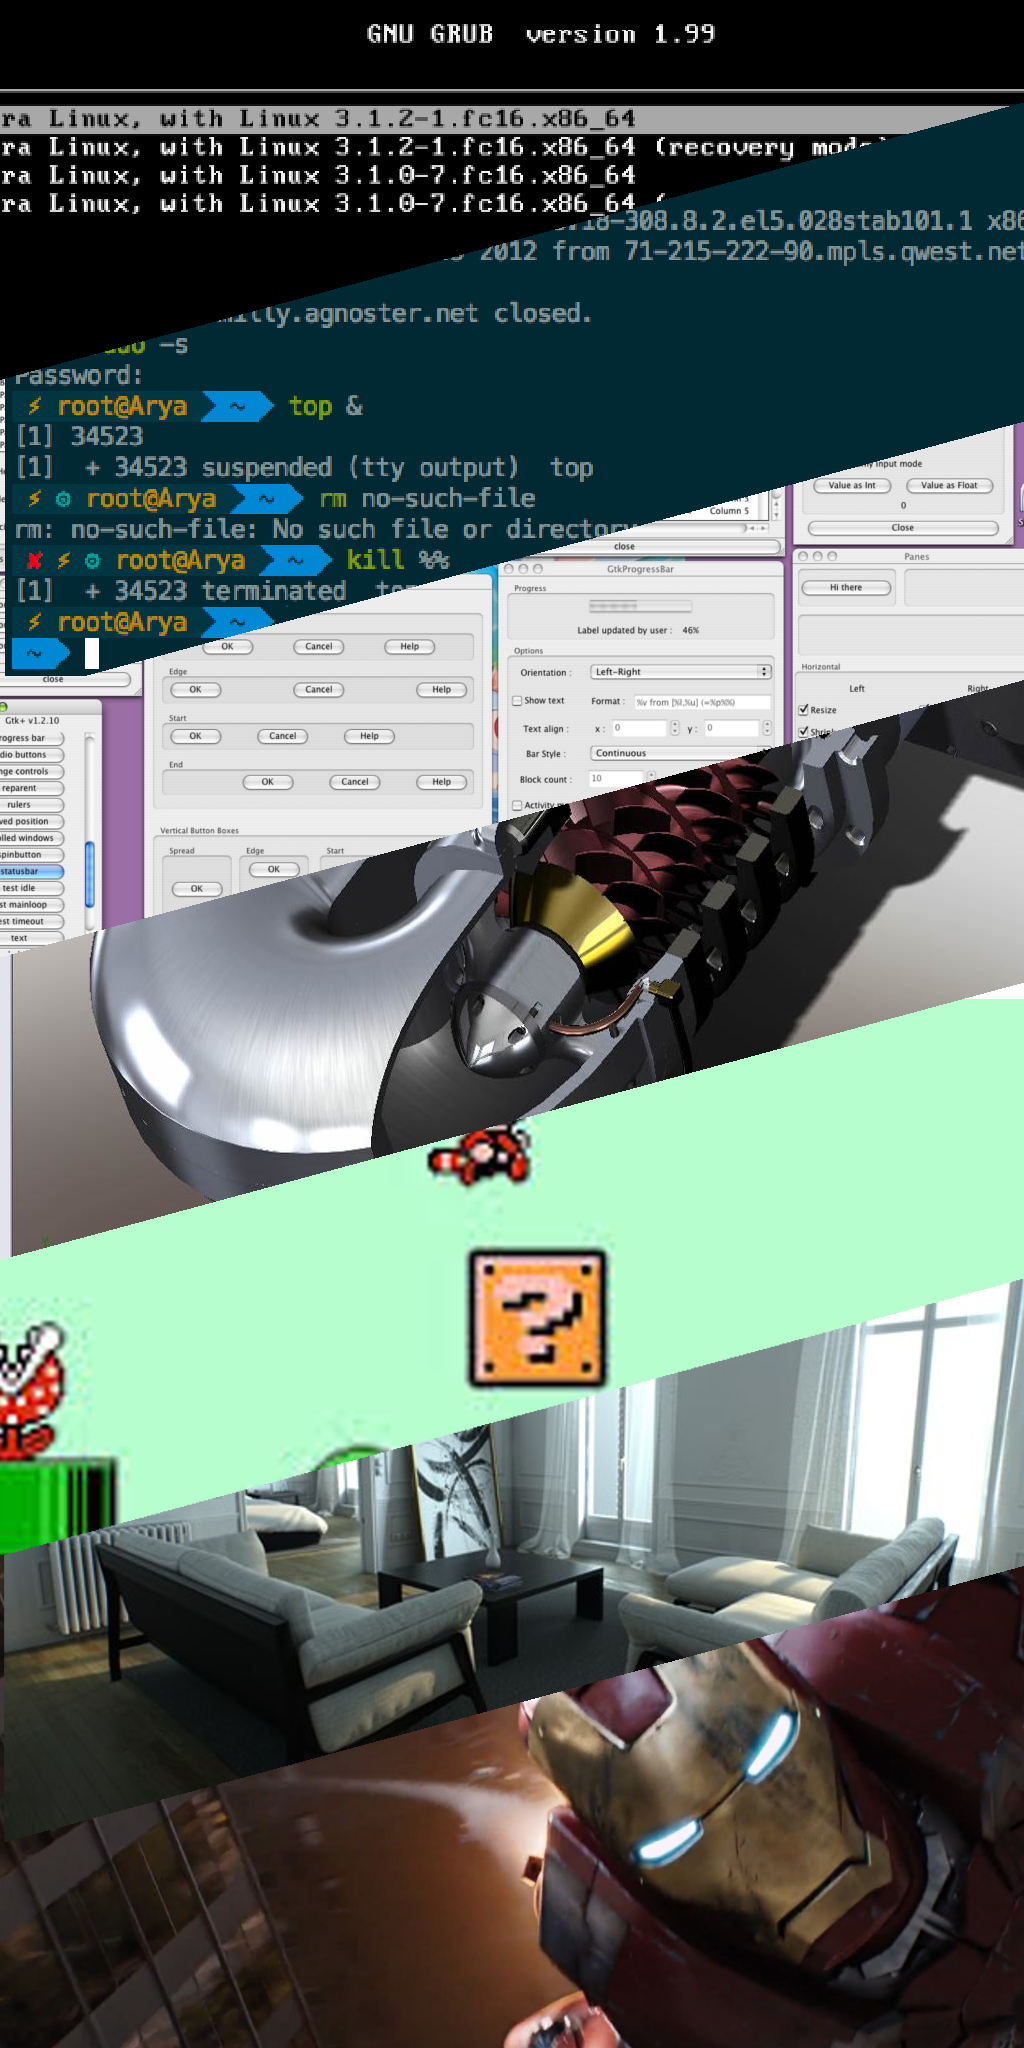
\includegraphics[width=\textwidth]{graphics/uses}}
    }
\end{frame}

\begin{frame}{Definition}
\begin{center}
    \pmidg{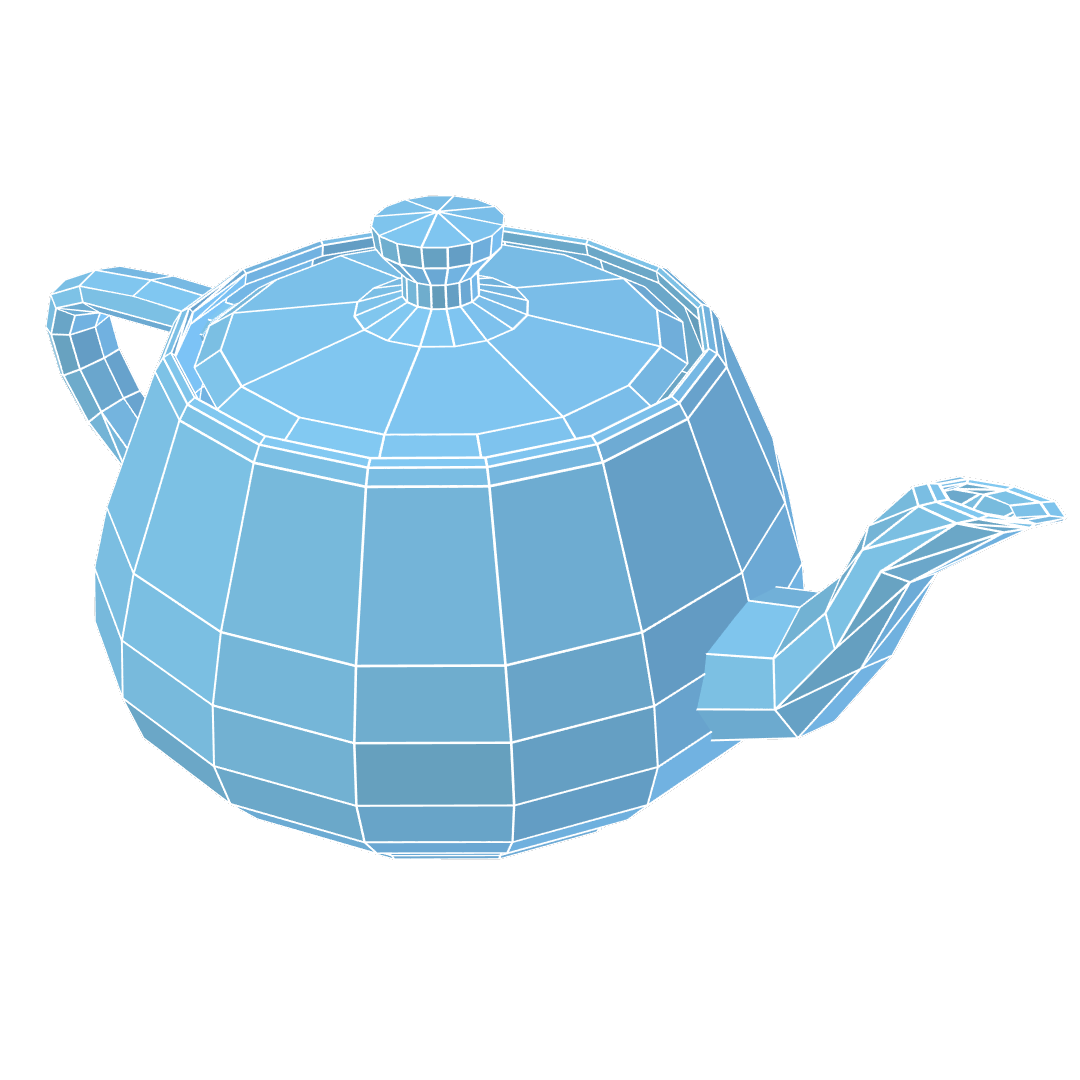
\includegraphics[width=4cm]{graphics/teapot_mesh}} \scalebox{2}{$\rightarrow$} \pmidg{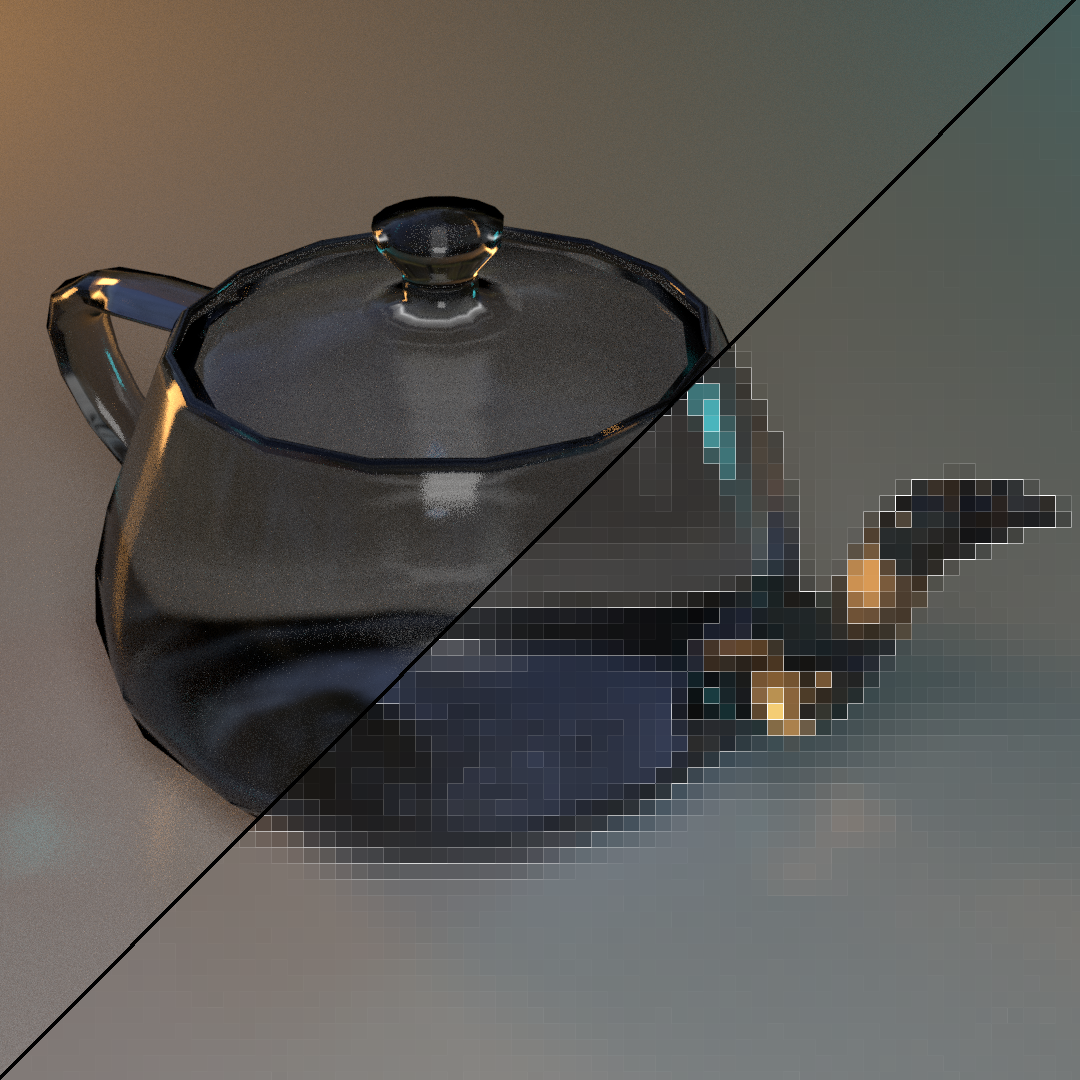
\includegraphics[width=4cm]{graphics/teapot_rt_pix}} \\
    
    \bigskip

    Computer graphics is the science of turning \textit{shapes} into \textit{pixels}. \footnote{Kindof, it can get more interesting than that}
\end{center}
\end{frame}

\section{Behind the Scenes}

\begin{frame}{Realtime}
    \splitslide{0.7}{.7em}{
        \small

        Realtime graphics use OpenGL or Direct3D to rasterize and shade
        triangular geometry on a graphics card/chip. Performance is very
        important due to the high framerate that is required for smooth
        gameplay/interactivity/animation. Lighting and materials focus on
        being "good enough" rather than on being truly accurate.

    }{
        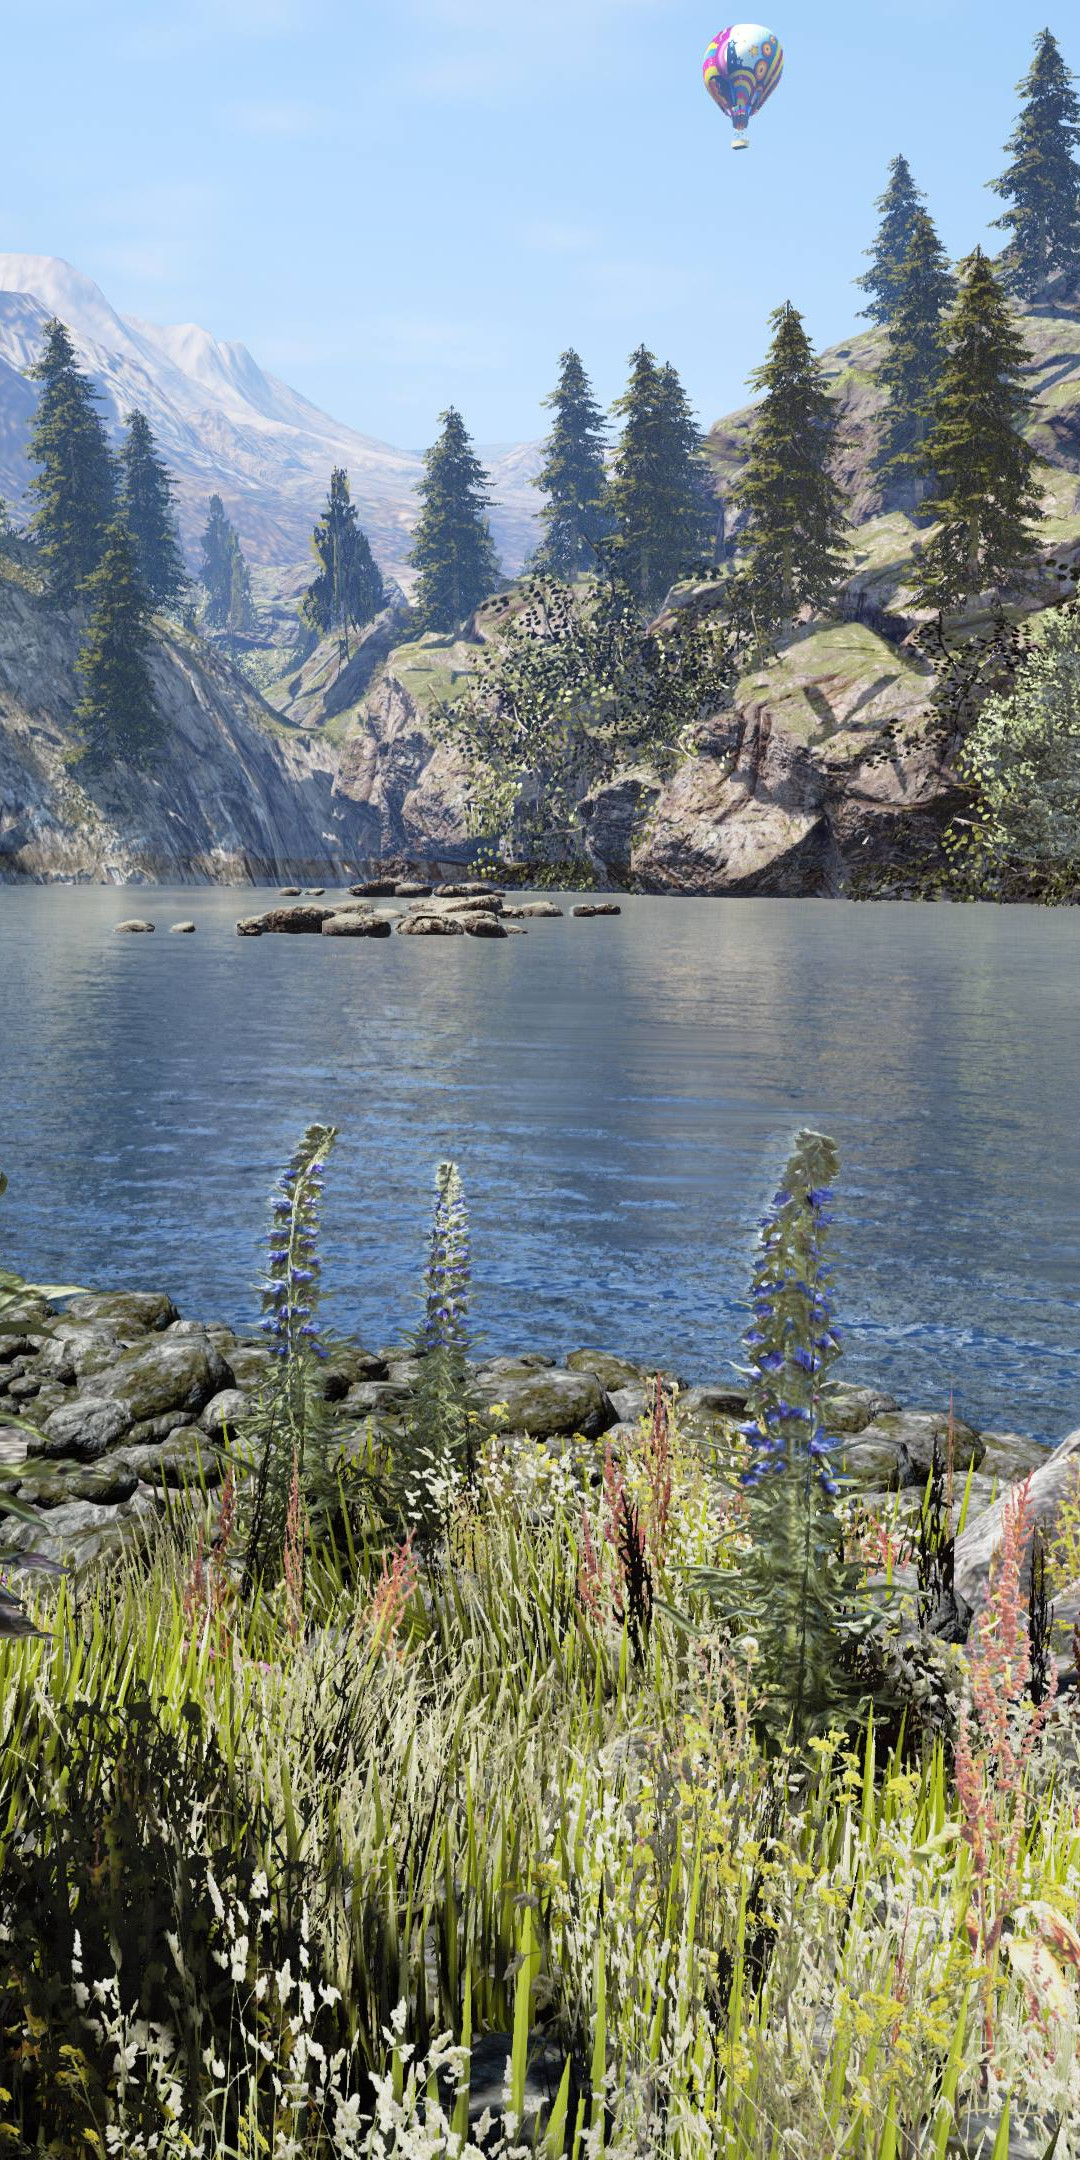
\includegraphics[width=\textwidth]{graphics/game_graphics}
    }
\end{frame}

\begin{frame}{UIs}
   \splitslide{0.7}{.7em}{
        \small

        While they look different, UIs generally use OpenGL or Direct3D as
        well. Everything is still made of textured \& shaded triangles. Anti-%
        aliasing, text fidelity, etc. are all more important while lighting
        effects are generally absent. Responsiveness is key, but the frame can
        be updated as needed, not every 30th of a second.

    }{
        
\includegraphics[width=\textwidth]{graphics/firefox_start}
    }
\end{frame}

\begin{frame}{Offline}
    \splitslide{0.7}{.7em}{
        \small

        Offline graphics are used when the medium is non-interactive (movies,
        advertisements, etc). Because the available resources are limited only
        by budget and patience, offline graphics have unmatched fidelity. CPUs
        are often used instead of GPUs because this allows for more advanced
        calculations. However, this comes at a cost. Individual frames may
        take days to render.

    }{
        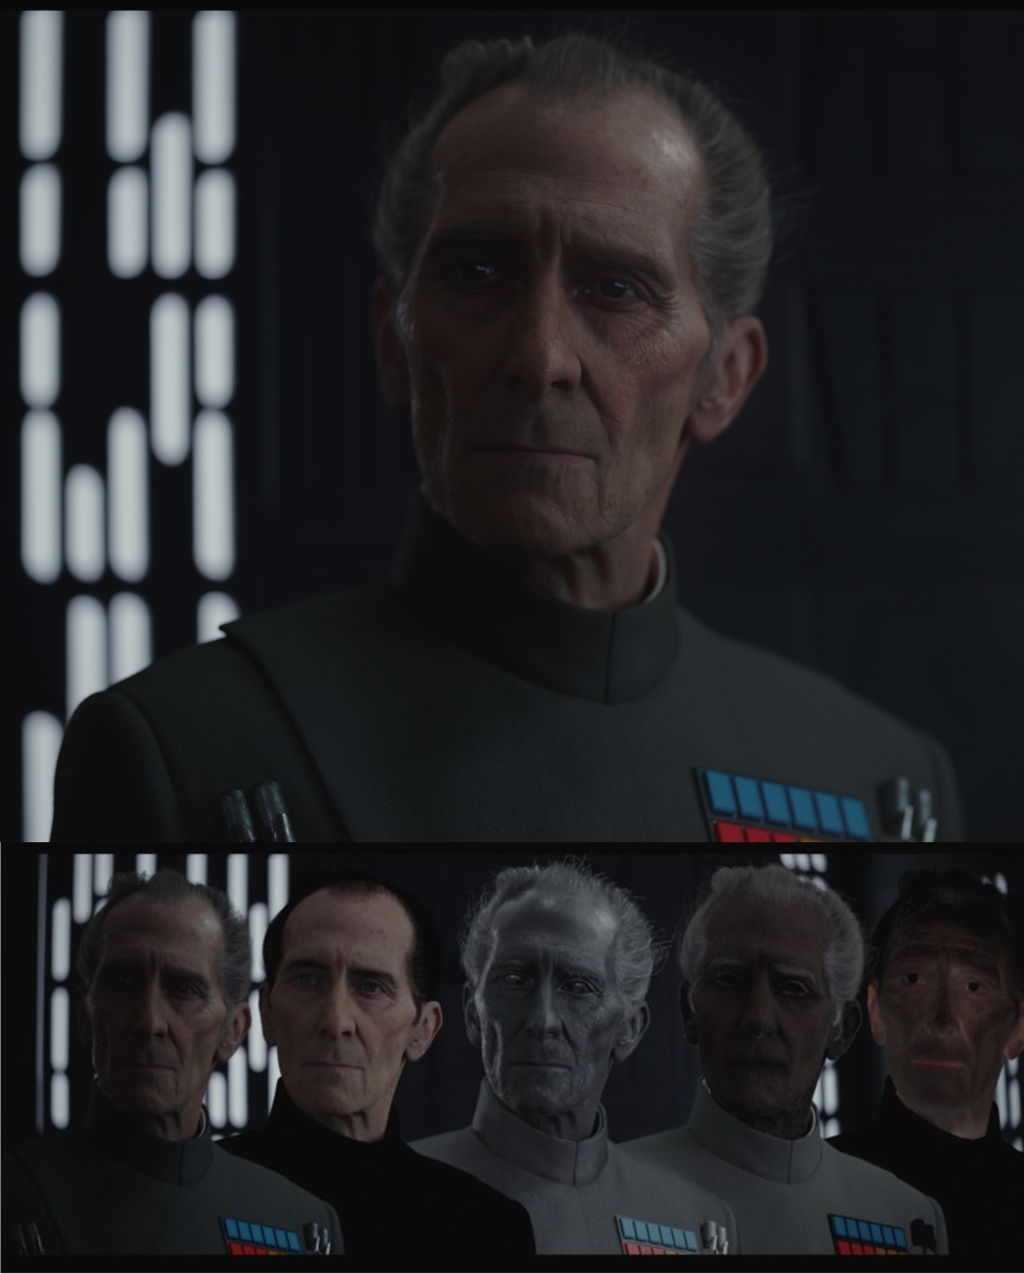
\includegraphics[width=\textwidth]{graphics/tarkin_combo} \\
        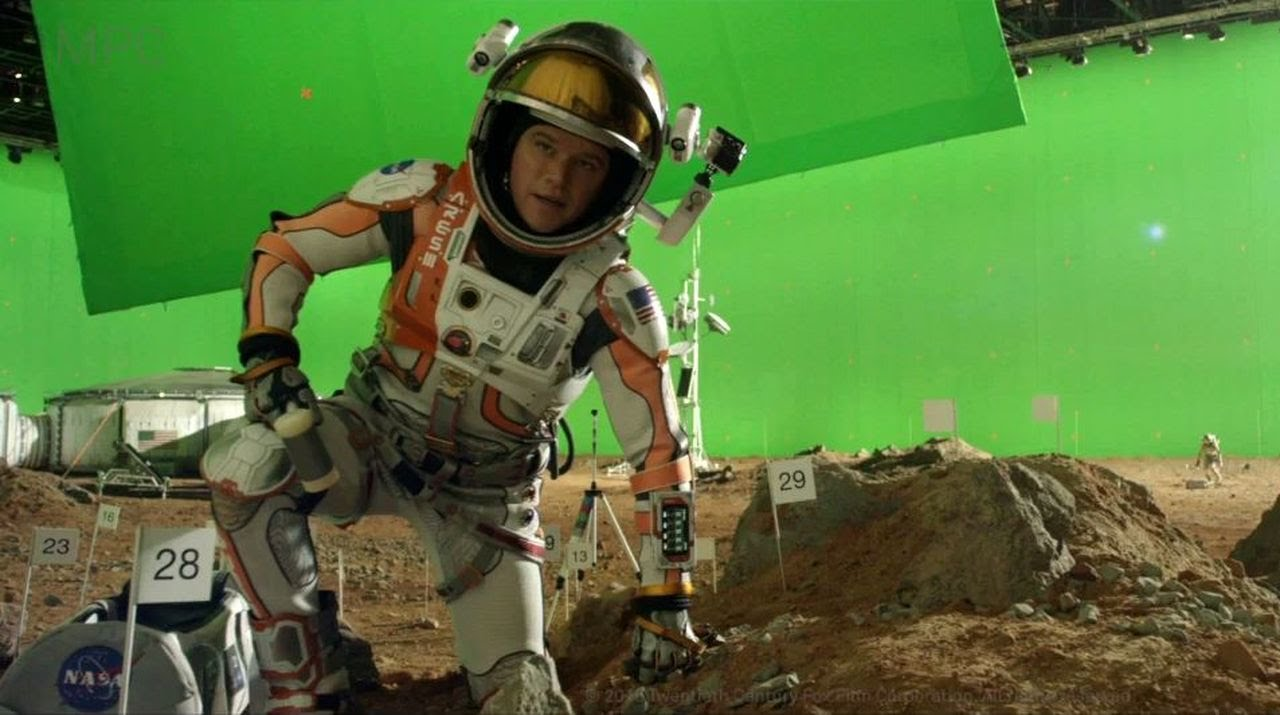
\includegraphics[width=\textwidth]{graphics/green_mars}
    }
\end{frame}

\section{History}

\begin{frame}{1950s \& 1960s}
    \splitslide{0.65}{.7em}{
        \small
        \begin{itemize}
            \item Military used computer controlled oscilloscopes to display strategic information
            \item Very simple graphical CAD programs and visualizers created
            \item Very first computer games
            \item Research into elementary 3D wireframe graphics
            \item Very early raster displays
        \end{itemize}
    }{
        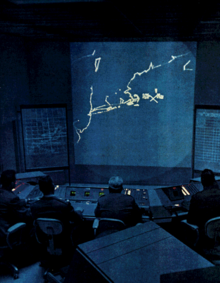
\includegraphics[width=\textwidth]{graphics/sage_control} \\
        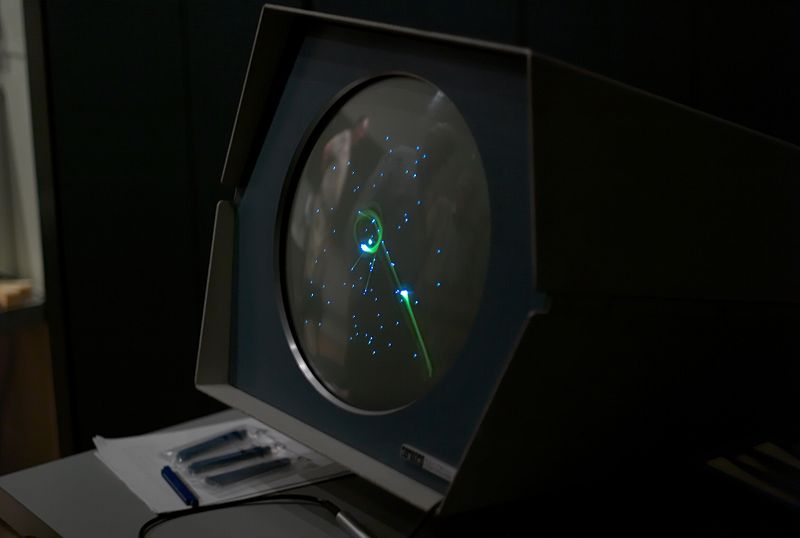
\includegraphics[width=\textwidth]{graphics/spacewar}
    }
\end{frame}

\begin{frame}{1970s \& 1980s}
    \splitslide{0.65}{.7em}{
        \small
        \begin{itemize}
            \item Basic lighting models such as Phong developed
            \item Low-res, 2D games become commercially available
            \item CGI starts to be used in Movies such as 1982's \textit{Wrath of Khan} and 1985's \textit{Young Sherlock Holmes}
            \item Modern GUIs are developed
            \item High-quality digital typesetting becomes commonplace
        \end{itemize}
    }{
        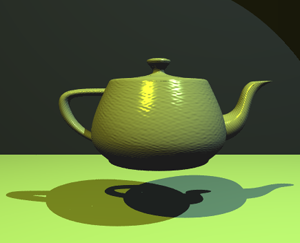
\includegraphics[width=\textwidth]{graphics/teapot_70s} \\
        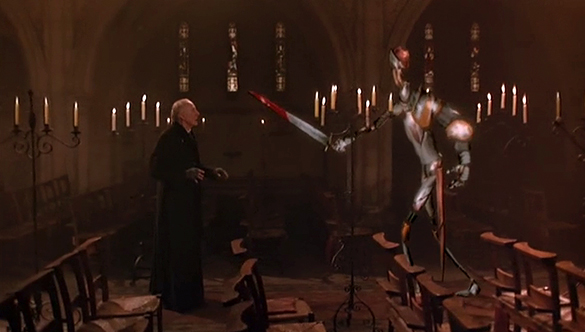
\includegraphics[width=\textwidth]{graphics/ysh_knight} \\
        
\includegraphics[width=\textwidth]{graphics/postscript_text}
    }
\end{frame}

\begin{frame}{1990s \& 2000s}
    \splitslide{0.65}{.7em}{
        \small
        \begin{itemize}
            \item Fidelity and performance are immensely increased
            \item Personal computers, 3D video games, and GUIs become ubiquitous
            \item OpenGL and Direct3D standardize hardware graphics support
            \item CGI becomes commonplace in Movies, advertisements, and TV 
            \item Global illumination and physically based rendering (PBR) techniques developed
        \end{itemize}
    }{
        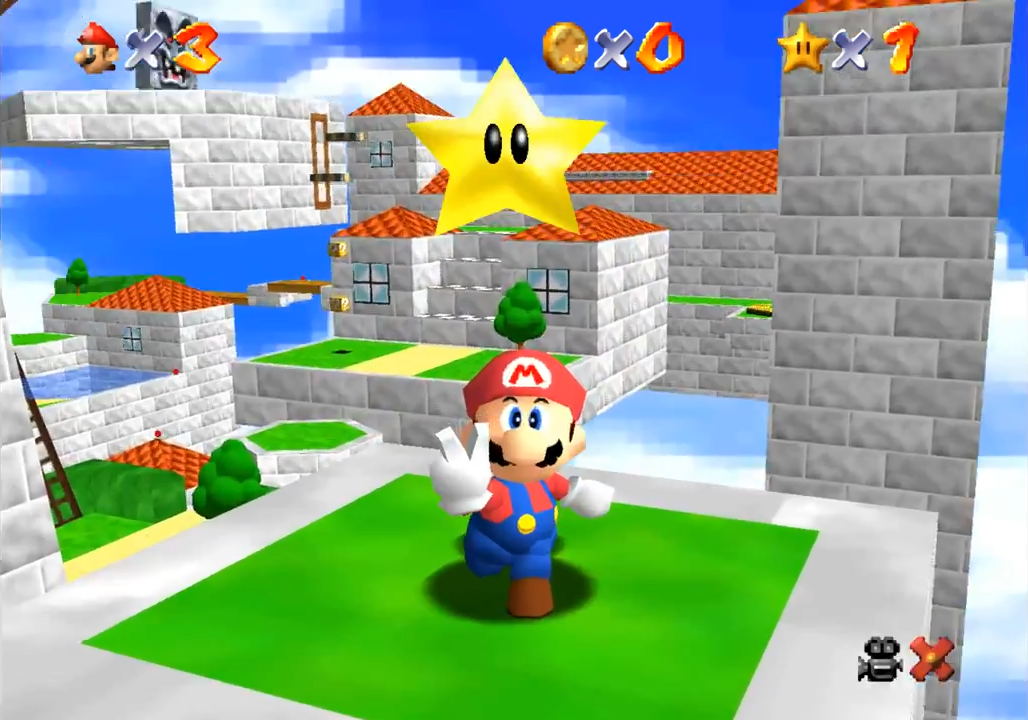
\includegraphics[width=\textwidth]{graphics/supermario64} \\
        
\includegraphics[width=\textwidth]{graphics/toy_story} \\
        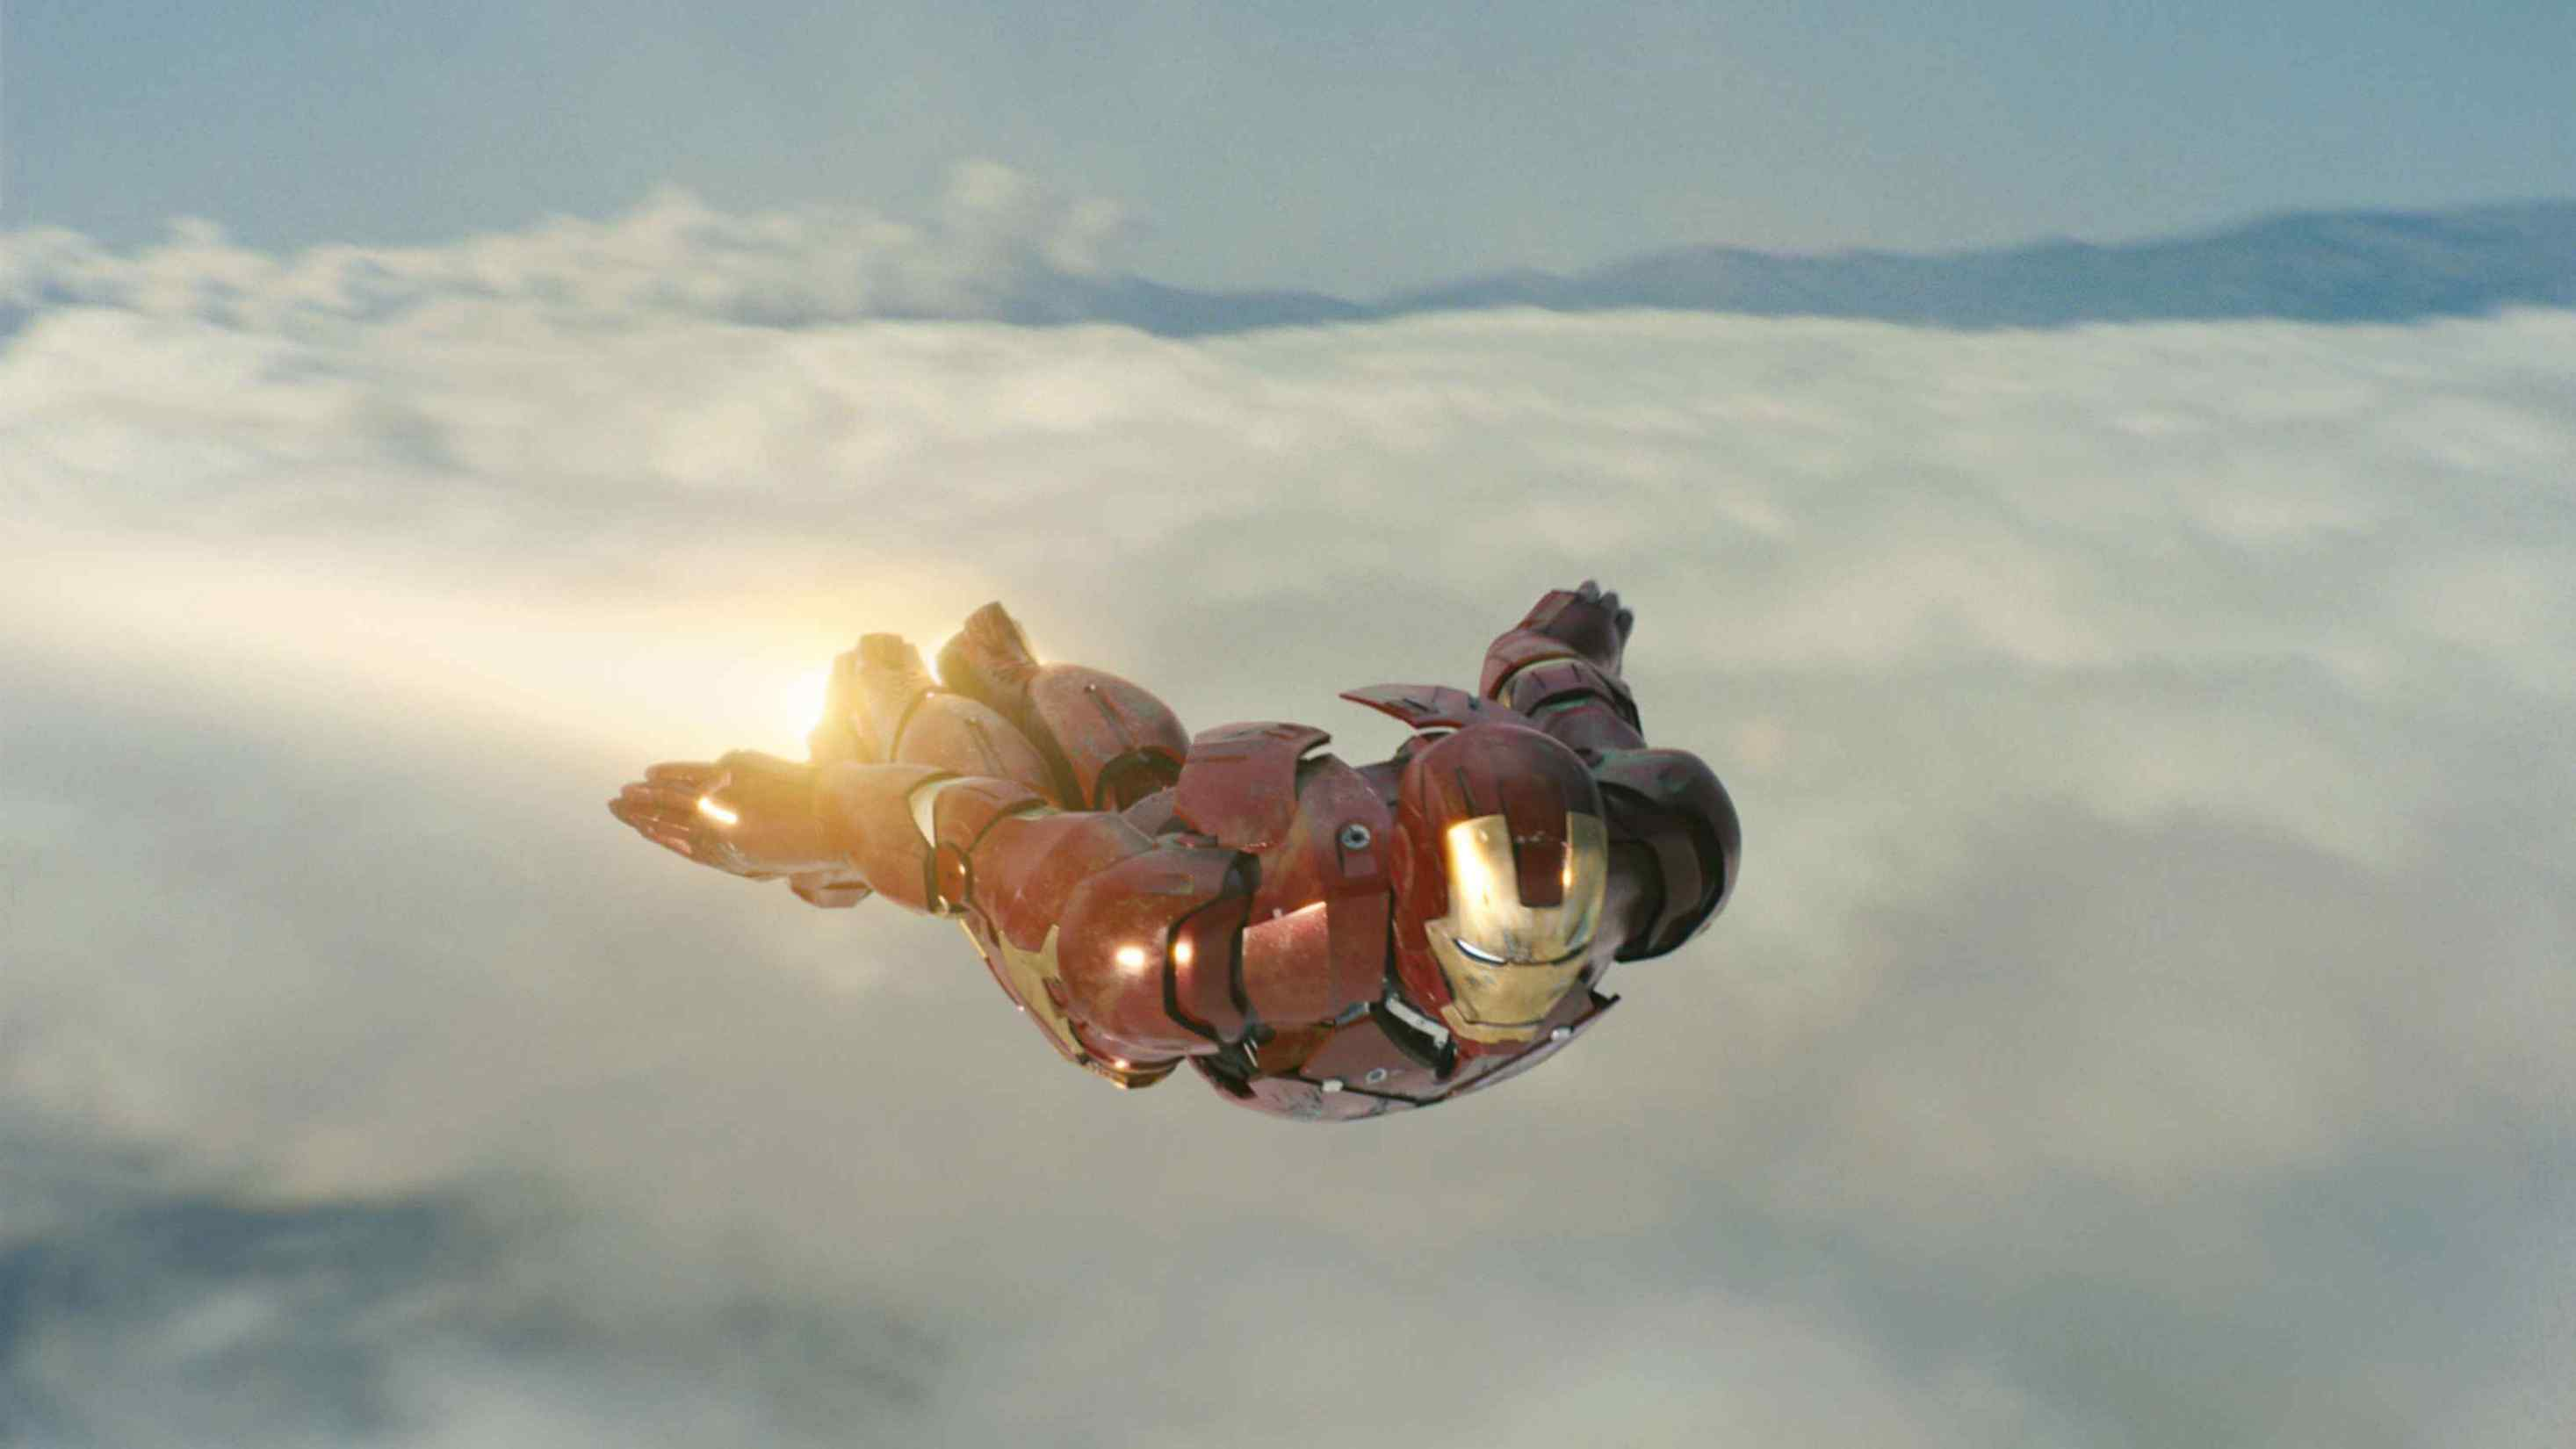
\includegraphics[width=\textwidth]{graphics/iron_man_2008}
    }
\end{frame}

\begin{frame}{Today}
    \splitslide{0.65}{.7em}{
        \small
        \begin{itemize}
            \item Given enough time, budget and expertise, offline graphics are photorealistic
            \item Particle and fluid simulations are extremely fast and accurate
            \item Realtime graphics make extensive use of shaders and PBR techniques
            \item UIs and offline graphics are increasingly GPU accelerated
            \item Linux and Mac have improved support for games and graphical software
        \end{itemize}
    }{
        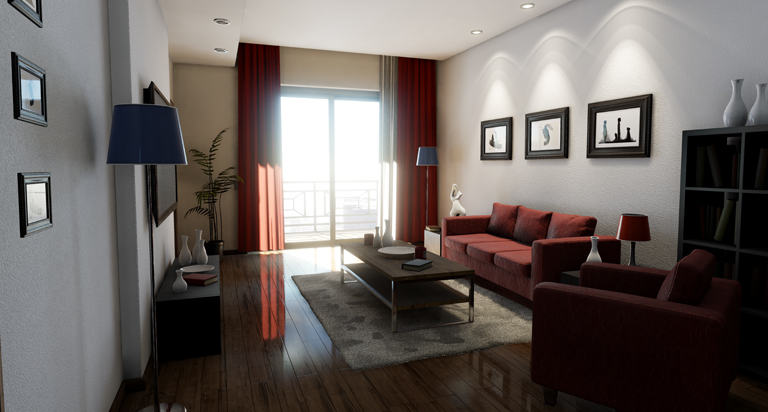
\includegraphics[width=\textwidth]{graphics/unreal4_damn.jpg} \\
        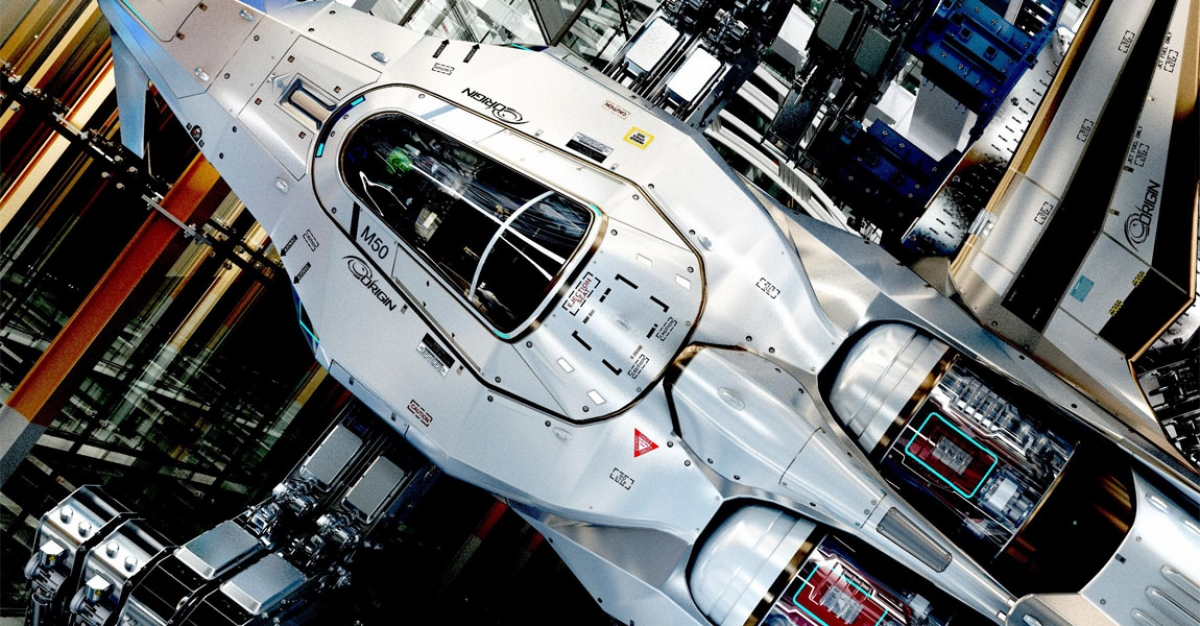
\includegraphics[width=\textwidth]{graphics/star_citizen_pbr} \\
        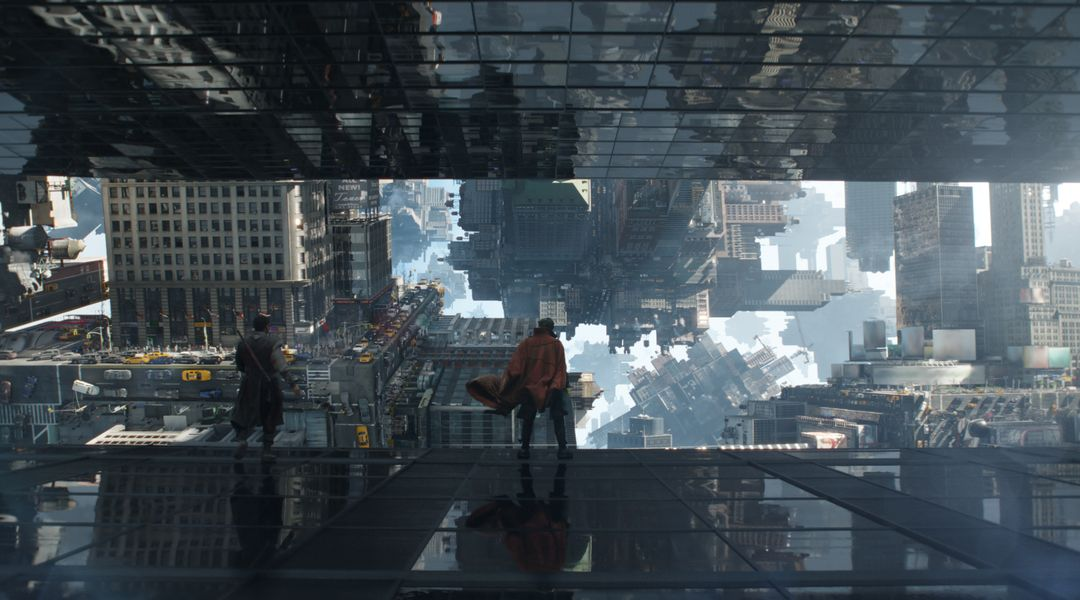
\includegraphics[width=\textwidth]{graphics/dr_strange} \\
        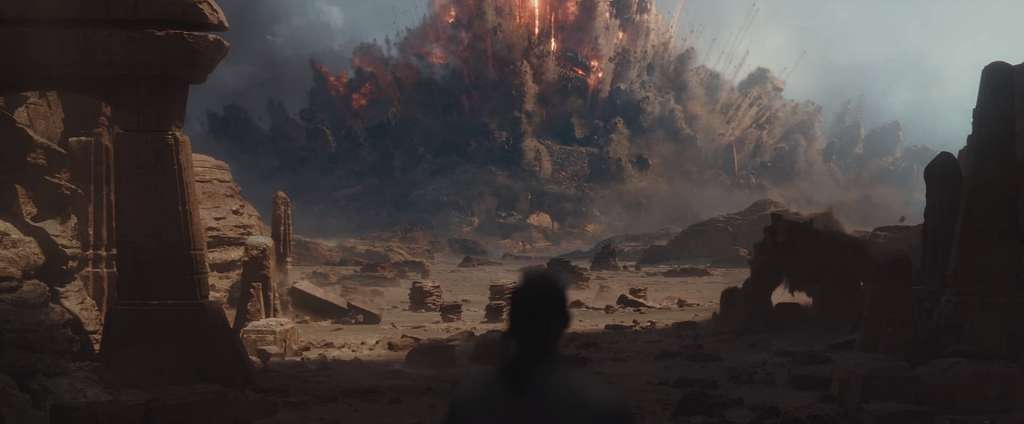
\includegraphics[width=\textwidth]{graphics/rogue_one_boom}
    }
\end{frame}

\section{Easy on the Eyes}

\begin{frame}{Text}
    \splitslide{0.65}{.7em}{
        \small

        The most common thing shown on screens is probably text. It is no
        wonder then that displaying text is one of the most sphisticated areas
        of computer graphics.

    }{
        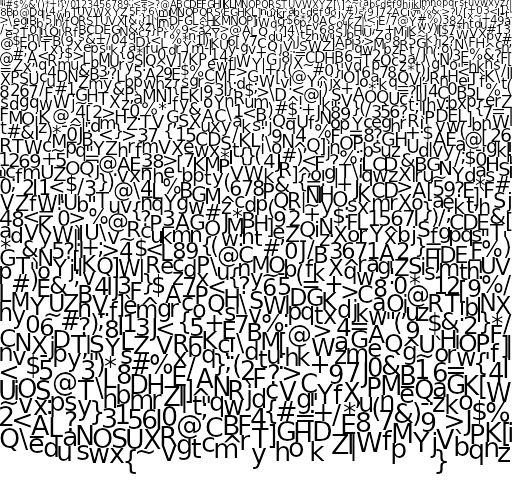
\includegraphics[width=\textwidth]{graphics/freetype_atlas} \\
        
\includegraphics[width=\textwidth]{graphics/subpixel_e}
    }
\end{frame}

\begin{frame}{Which is better?}
    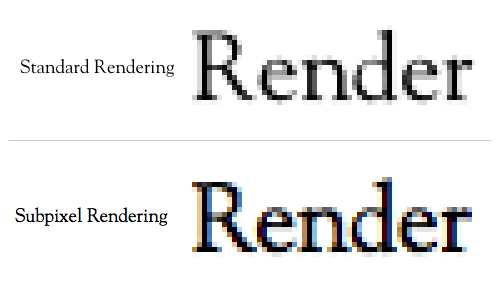
\includegraphics[width=\textwidth]{graphics/subpixel_side_by_side}
\end{frame}

\begin{frame}{Anti-aliasing}
    \splitslide{0.65}{.7em}{
        \small

        When small shapes (such as letters) are rasterized, details can find
        themselves squished into single pixels. In these cases, the color of
        the pixel is chosen arbitrarily depending on how the rasterization is
        performed. This creates all sorts of strange effects and hard edges,
        called "aliases".

        \vspace{1ex}

        The quality of the image can be greatly improved in some cases by
        using "anti-aliasing" algorithms and techniques.

    }{
        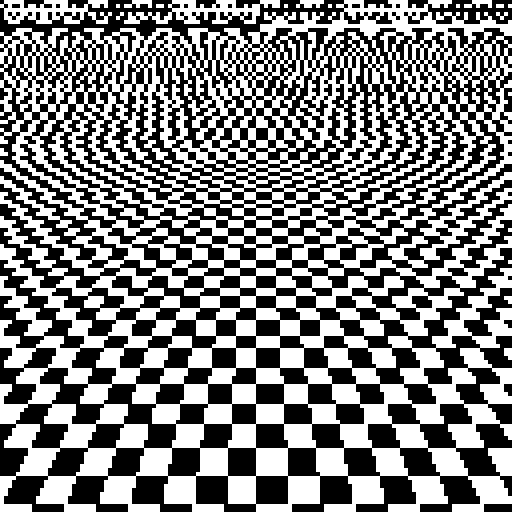
\includegraphics[width=\textwidth]{graphics/aliased} \\
        
\includegraphics[width=\textwidth]{graphics/antialias_line}
    }
\end{frame}

\begin{frame}{Sub-pixels}
    \splitslide{0.65}{.7em}{
        \small

        Anti-aliasing can be taken further. After all, each pixel is really 3
        small red, green, and blue rectangles joined together. Clever people
        have figured out how to use these extra rectangles to further smooth
        the edges of letters and lines. This is why blown-up text (in an image
        editor) ends up being slightly colored on the edges.

    }{
        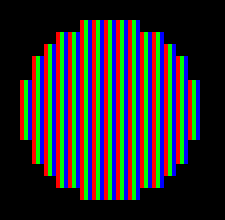
\includegraphics[width=\textwidth]{graphics/pixel_circle} \\
        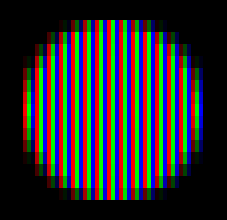
\includegraphics[width=\textwidth]{graphics/subpixel_circle}
    }
\end{frame}

\section{3D Shapes \& Geometry}

\begin{frame}{Meshes}
    \splitslide{0.65}{.7em}{
        \small

        3D shapes are often stored as a jumble of points (called verticies),
        scattered in space. These points are linked together into polygons,
        which form the surface of the model. Other methods of storing 3D
        shapes exist, such as the parametric forms used by Solid Works, but
        "meshes" are by far the most common. In fact, even when a different
        form is used, the model is almost always converted into a mesh for
        rendering anyway.

    }{
        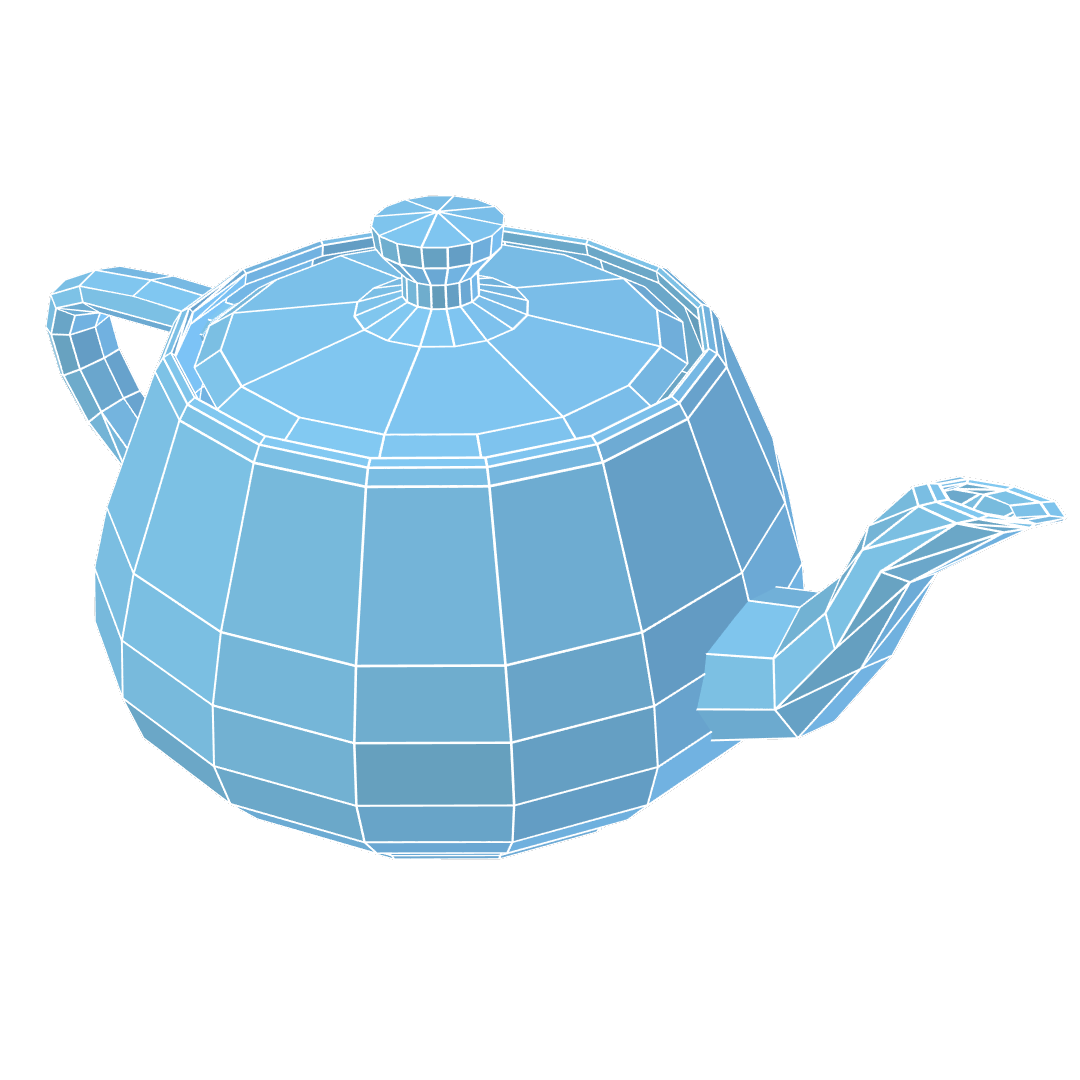
\includegraphics[width=\textwidth]{graphics/teapot_mesh}
    }
\end{frame}

\begin{frame}{Triangles}
    \splitslide{0.65}{.7em}{
        \small

        While any polygon could be used in a mesh, modern computer graphics
        deal almost exclusively in triangles. This is because triangles have
        some nice geometric properties that other shapes don't:

        \begin{itemize}
            \item It is very easy to test if a point is within a triangle (barycentric coordinates!)
            \item Any 3 points can be haphazardly connected together and still form a \underline{flat} triangle
            \item It is easy to calculate the direction a triangle is facing
        \end{itemize}
    }{
        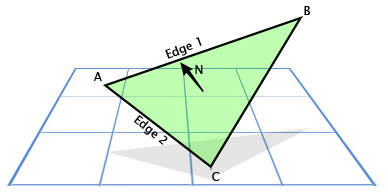
\includegraphics[width=\textwidth]{graphics/triangle}
    }
\end{frame}

\begin{frame}{3D Modeling}
    \splitslide{0.5}{.2em}{
        
\includegraphics[width=\textwidth]{graphics/subpixel_e}
    }{
        
\includegraphics[width=\textwidth]{graphics/subpixel_e}
    }
\end{frame}

\section{Making it Pretty}

\begin{frame}{Textures}
    \splitslide{0.65}{.7em}{
        \small

         Textures are images (though they can contain more than colors) that
         are wrapped around 3D models. The exact method for this varies, but
         most of the time the wrapping is defined by a second set of
         coordinates attached to each vertex/point. This specifies where on
         the texture that point (and by extension, attached triangles) should
         lie.

         \vspace{1ex}

         This second set of positions is called the "UV map".

    }{
        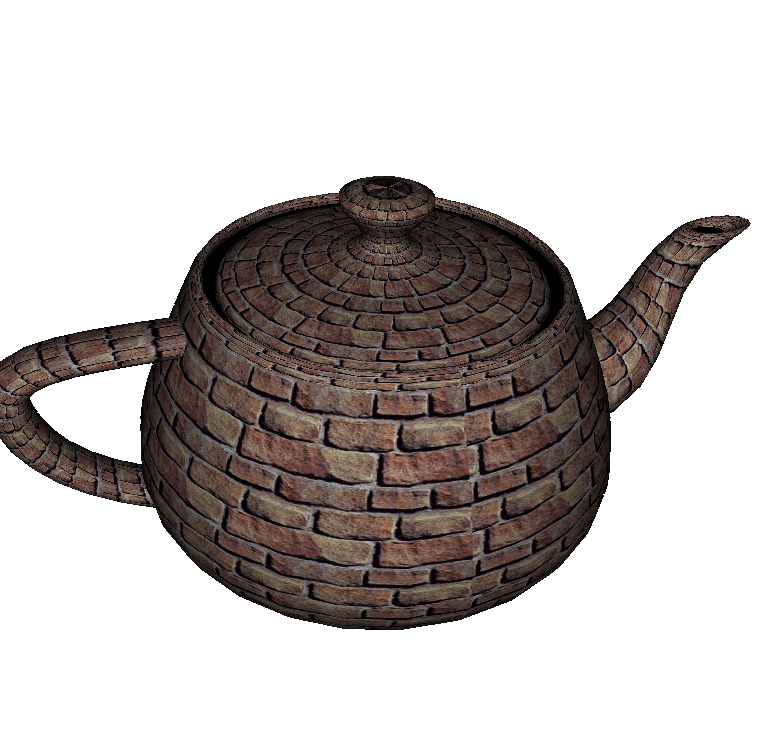
\includegraphics[width=\textwidth]{graphics/teapot_brick} \\
        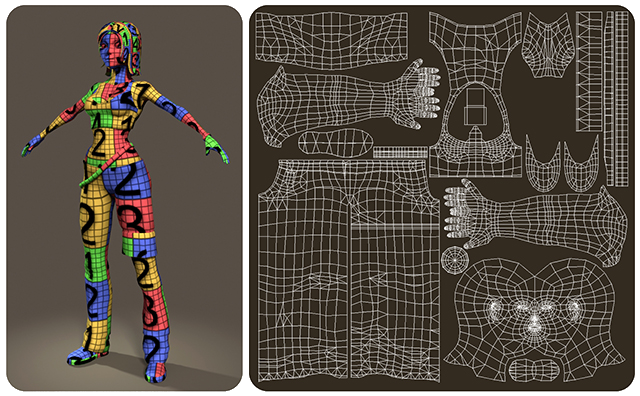
\includegraphics[width=\textwidth]{graphics/uv_map}
    }
\end{frame}

\begin{frame}{Mapping}
    \splitslide{0.65}{.7em}{
        \small

        Textures can be used to cover objects in all sorts of information. Not
        just color, but also material properties such as shininess and even
        precaculated lighting information.

        \vspace{1ex}

        More advanced techniques (such as bump, normal, and parallax mapping)
        can be used to fake bumps and other minute, shaded details on
        technically flat surfaces. Games use this extensively to make low-%
        resolution objects appear highly detailed (think screws, buckles,
        bricks, tree bark, ground texture, etc.)
 
    }{
        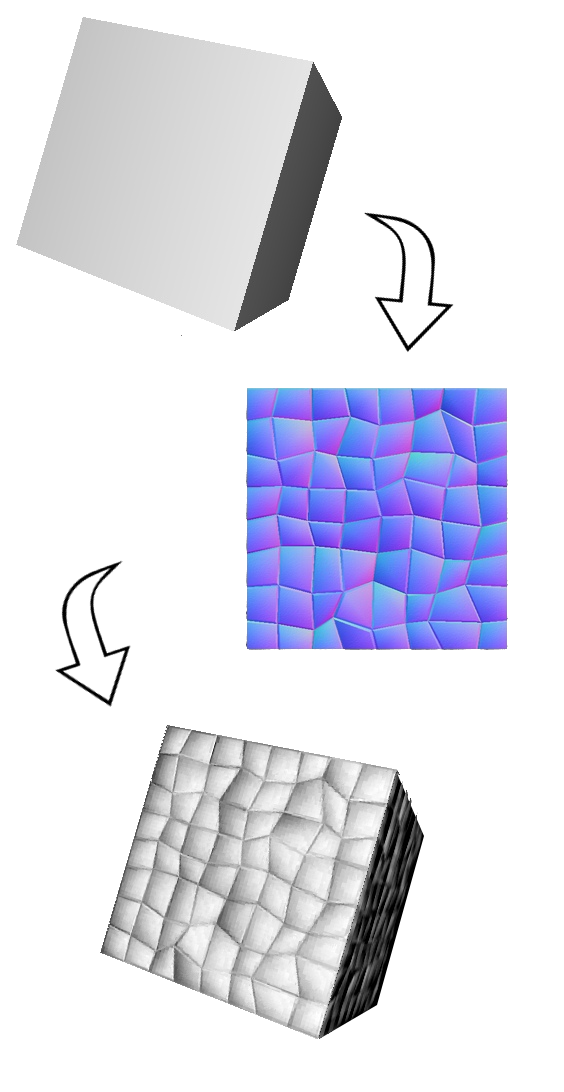
\includegraphics[width=\textwidth]{graphics/normal_map}
    }
\end{frame}

\begin{frame}{Phong}
    \splitslide{0.65}{.7em}{
        \small

        Phong is the simplest common shading model. It mixes diffuse shading
        (areas facing a light are brighter) and specular shading (areas that
        reflect light towards the camera are brighter) together. Think of how
        you would shade something with a pencil.

        \vspace{1ex}

        While this kind of works, it massively simplifies how real-world
        materials and lights interact. As a result, it looks downright fake.

    }{
        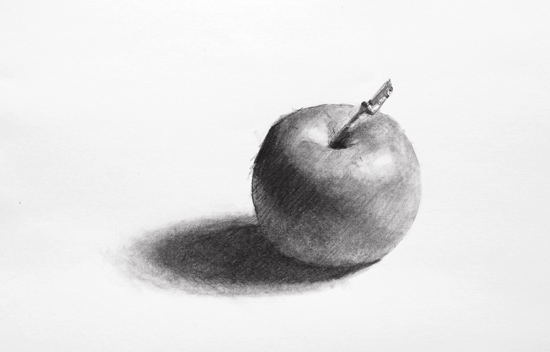
\includegraphics[width=\textwidth]{graphics/pencil_phong} \\
        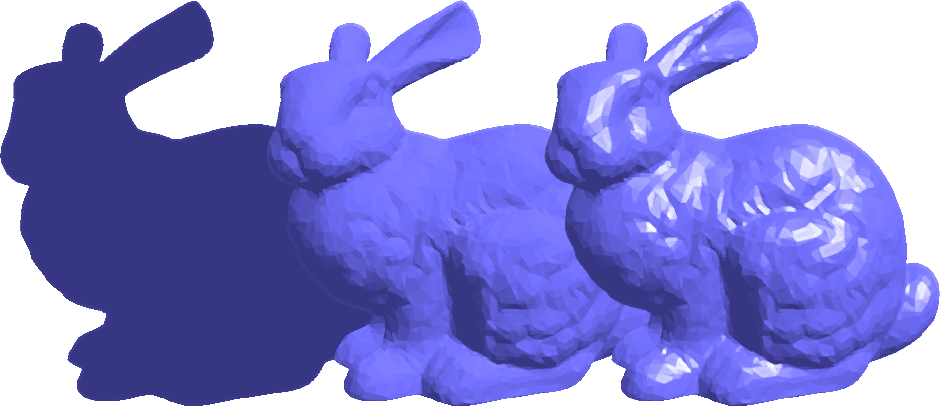
\includegraphics[width=\textwidth]{graphics/phong}
    }
\end{frame}

\begin{frame}{Painter's Algorithm}
    \splitslide{0.65}{.7em}{
        \small

        It goes without saying that things that are farther away should be
        hidden by things that are closer. The simplest way to do this in a
        computer is to draw the farther stuff first, so that when nearer stuff
        is drawn, it covers the previous stuff up.

        \vspace{1ex}

        However, this requires all the objects in the scene to be constantly
        resorted. It also can't deal with objects that mutually cover each
        other (like the Olympic rings).

        \vspace{1ex}

        That being said, there are still cases where the Painter's Algorithm
        is the only viable method.

    }{
        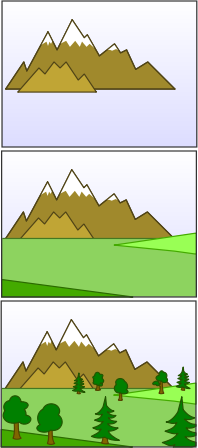
\includegraphics[width=\textwidth]{graphics/painters_alg}
    }
\end{frame}

\begin{frame}{Depth}
    \splitslide{0.65}{.7em}{
        \small

        A more common way to hide objects behind each other is to use a depth
        buffer. A depth buffer is a sort of distance image. In addition to
        keeping track of the color of each pixel, the distance from the camera
        to that pixel is also tracked. Then, whenever a new pixel is
        calculated, the computer checks whether is in front of or behind what
        is already there.

    }{
        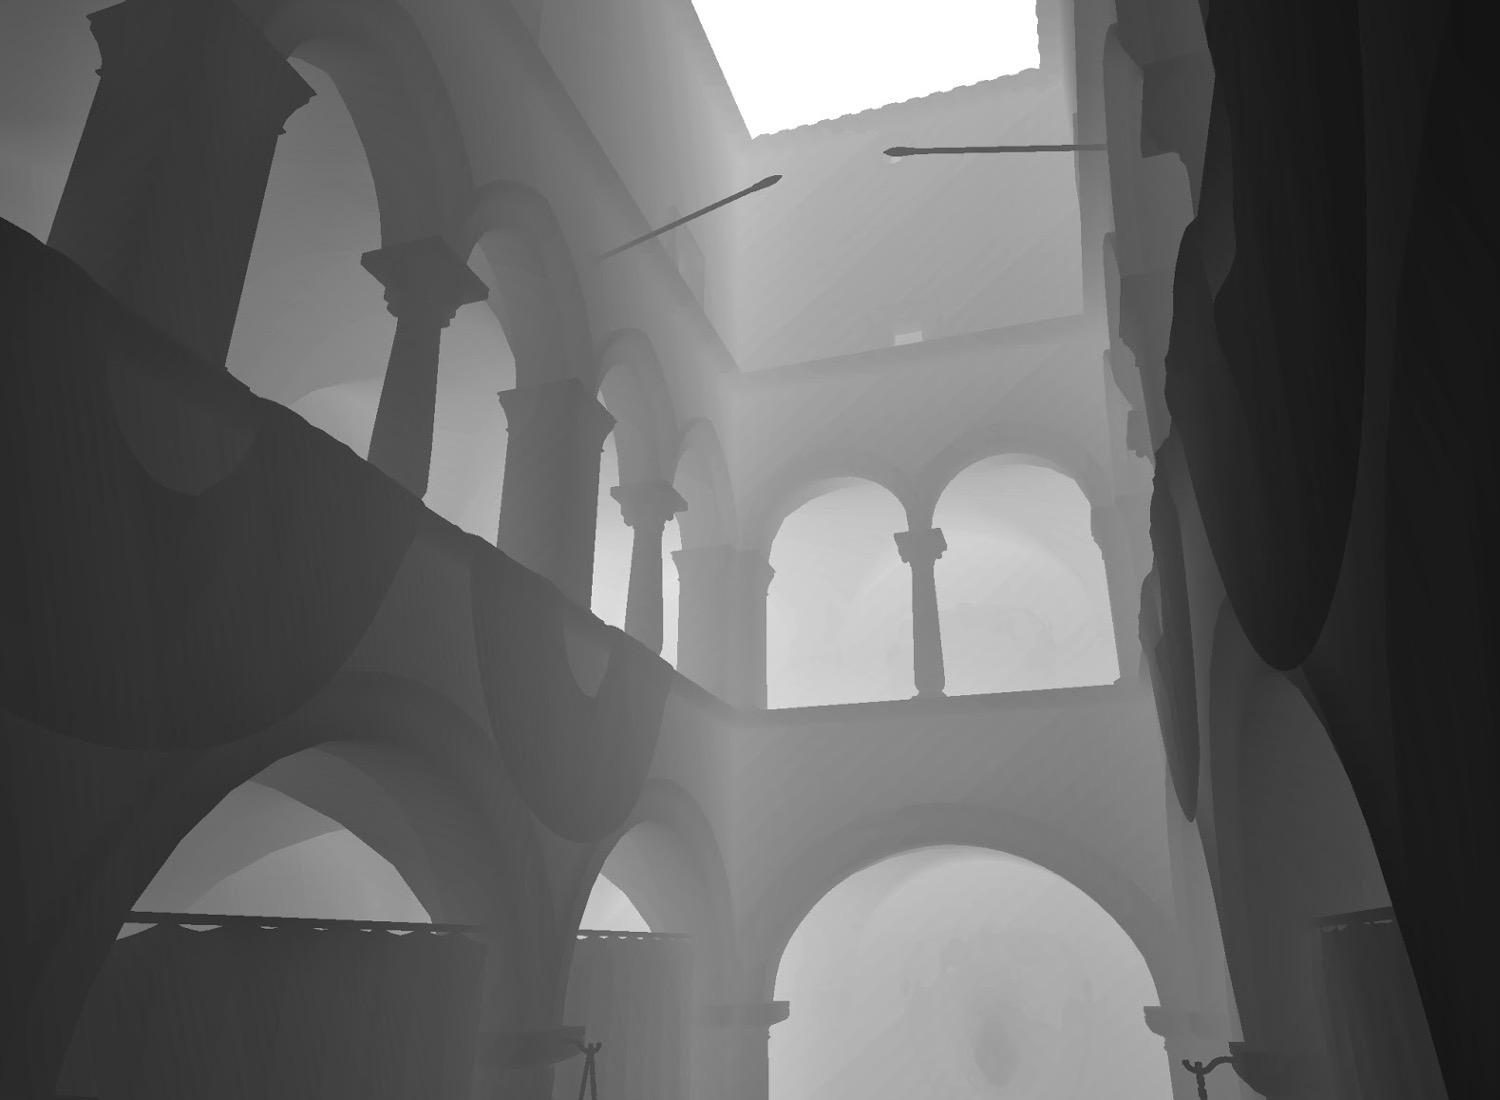
\includegraphics[width=\textwidth]{graphics/zbuffer2} \\
        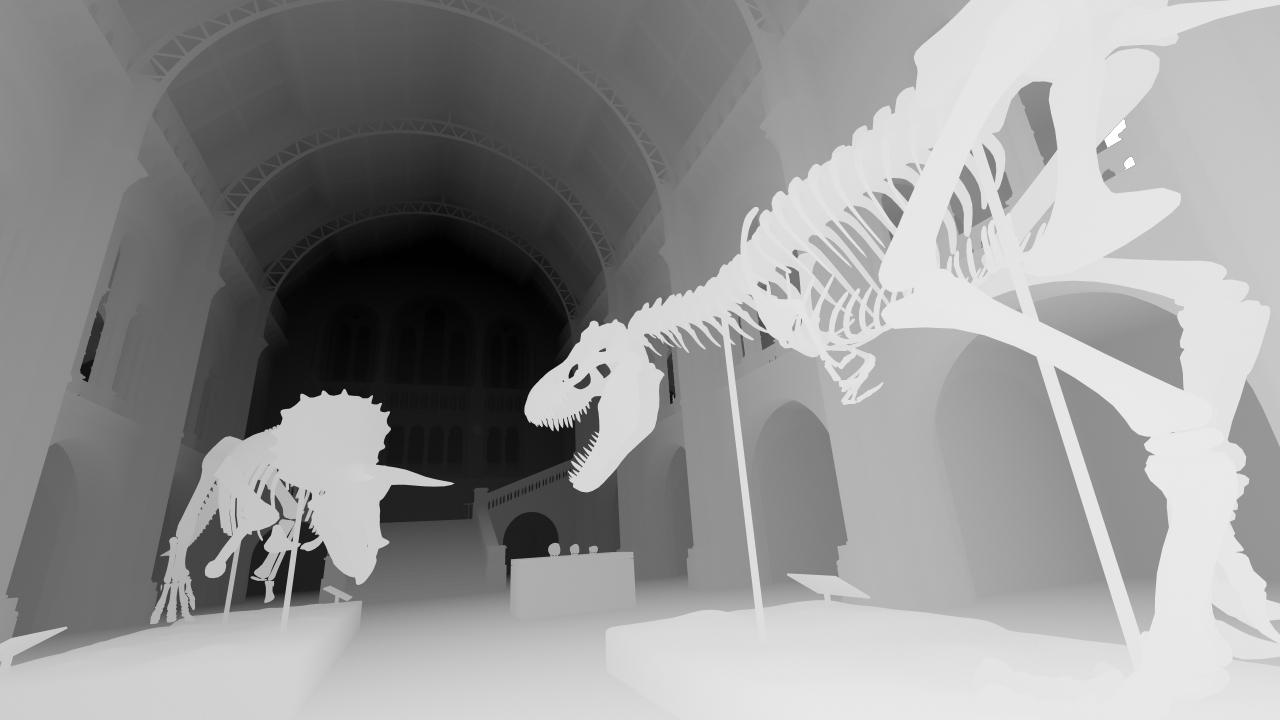
\includegraphics[width=\textwidth]{graphics/zbuffer}
    }
\end{frame}

\section{Effects}

\begin{frame}{Transparency}
    \splitslide{0.65}{.7em}{
        \small

        Transparency can put a wrench in things.

    }{
        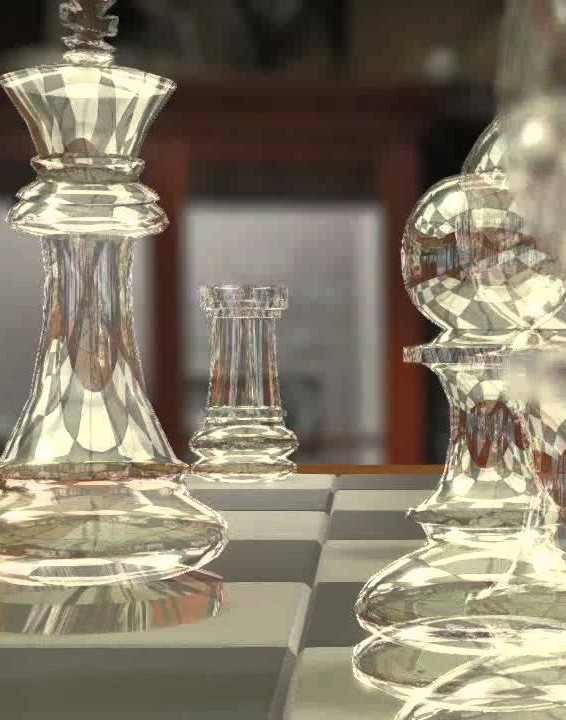
\includegraphics[width=\textwidth]{graphics/transparent}
    }
\end{frame}

\begin{frame}{Post-Processing}
    \splitslide{0.65}{.7em}{
        \small

        Texturing and shading is not always enough to make an image look good.
        Any photoshop guru can tell you how much a little tweaking can improve
        things. These "post-processing effects" arn't just used to make
        realtime graphics nicer, they are used to style-up photographs and
        videos as well.

    }{
        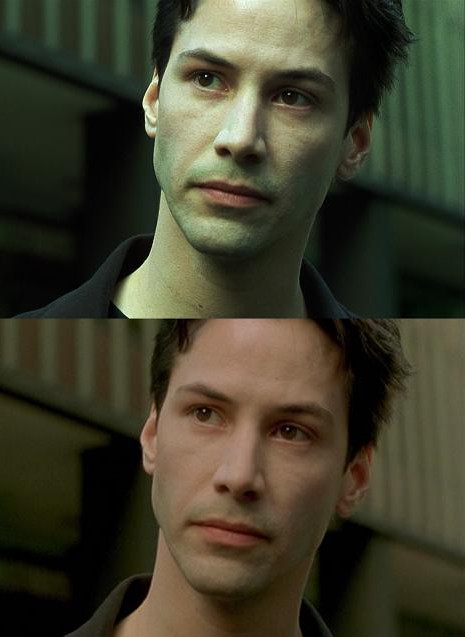
\includegraphics[width=\textwidth]{graphics/color_grading.jpeg}
    }
\end{frame}

\begin{frame}{Multipass Rendering}
    \splitslide{0.65}{.7em}{
        \small

        Post-processing can be taken even further. Instead of lighting and
        textured being performed as the shapes are rasterized, data from along
        the way can be saved in buffers and stapled together after the fact.

        \vspace{1ex}

        This has numerous benefits depending on how it is used. It is useful
        in realtime graphics because data from a single pass can be recycled
        to create multiple effects. Artists working on offline graphics like
        it because it lets them tweak shading and lighting without re-%
        rendering the whole scene.

    }{
        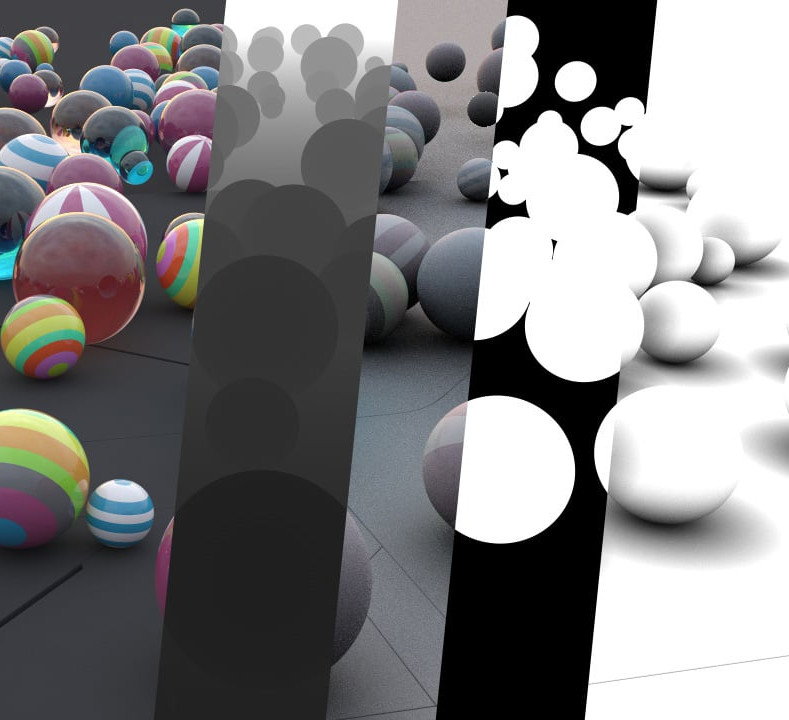
\includegraphics[width=\textwidth]{graphics/multipass}
    }
\end{frame}

\begin{frame}{Bluring}
    \splitslide{0.65}{.7em}{
        \small

        Transparency can put a wrench in things.

    }{
        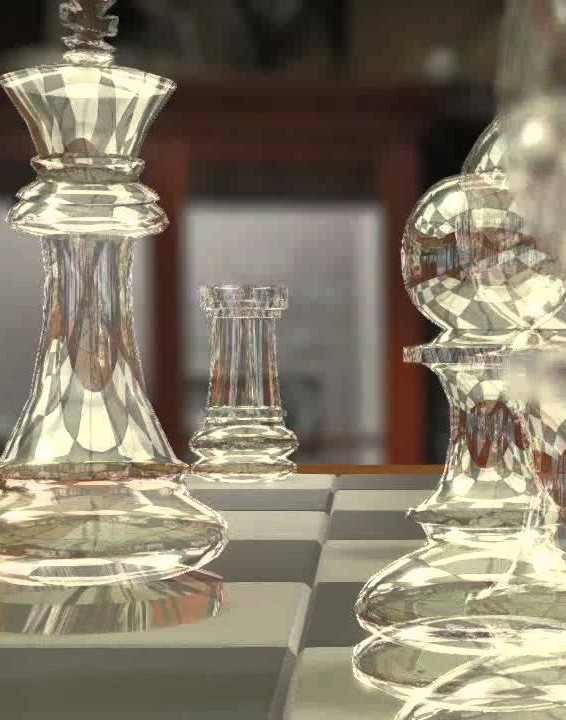
\includegraphics[width=\textwidth]{graphics/transparent}
    }
\end{frame}

\begin{frame}{Compositing}
    \splitslide{0.65}{.7em}{
        \small
        \begin{itemize}
            \item ...
        \end{itemize}
    }{
        
\includegraphics[width=\textwidth]{graphics/subpixel_e}
    }
    \noindent
\end{frame}

\section{Realism}

\begin{frame}{Reflection}
    \splitslide{0.65}{.7em}{
        \small
        \begin{itemize}
            \item ...
        \end{itemize}
    }{
        
\includegraphics[width=\textwidth]{graphics/subpixel_e}
    }
\end{frame}

\begin{frame}{Refraction}
    \splitslide{0.65}{.7em}{
        \small
        \begin{itemize}
            \item ...
        \end{itemize}
    }{
        
\includegraphics[width=\textwidth]{graphics/subpixel_e}
    }
\end{frame}

\begin{frame}{Raytracing}
    \splitslide{0.65}{.7em}{
        \small
        \begin{itemize}
            \item ...
        \end{itemize}
    }{
        
\includegraphics[width=\textwidth]{graphics/subpixel_e}
    }
\end{frame}

\begin{frame}{Fresnel \& PBR}
    \splitslide{0.65}{.7em}{
        \small
        \begin{itemize}
            \item ...
        \end{itemize}
    }{
        
\includegraphics[width=\textwidth]{graphics/subpixel_e}
    }
\end{frame}

\begin{frame}{Local Illumination}
    \splitslide{0.65}{.7em}{
        \small
        \begin{itemize}
            \item ...
        \end{itemize}
    }{
        
\includegraphics[width=\textwidth]{graphics/subpixel_e}
    }
\end{frame}

\begin{frame}{Global Illumination}
    \splitslide{0.65}{.7em}{
        \small
        \begin{itemize}
            \item ...
        \end{itemize}
    }{
        
\includegraphics[width=\textwidth]{graphics/subpixel_e}
    }
\end{frame}

\begin{frame}{Pathtracing}
    \splitslide{0.65}{.7em}{
        \small
        \begin{itemize}
            \item ...
        \end{itemize}
    }{
        
\includegraphics[width=\textwidth]{graphics/subpixel_e}
    }
    \noindent
\end{frame}

\section{Wrapping it Up}

\end{document}